\documentclass{standalone}
\usepackage{graphicx}	
\usepackage{amssymb, amsmath}
\usepackage{color}

\usepackage{tikz}
\usetikzlibrary{intersections, backgrounds}

\definecolor{light}{RGB}{220, 188, 188}
\definecolor{mid}{RGB}{185, 124, 124}
\definecolor{dark}{RGB}{143, 39, 39}
\definecolor{highlight}{RGB}{180, 31, 180}
\definecolor{gray10}{gray}{0.1}
\definecolor{gray20}{gray}{0.2}
\definecolor{gray30}{gray}{0.3}
\definecolor{gray40}{gray}{0.4}
\definecolor{gray60}{gray}{0.6}
\definecolor{gray70}{gray}{0.7}
\definecolor{gray80}{gray}{0.8}
\definecolor{gray90}{gray}{0.9}
\definecolor{gray95}{gray}{0.95}

\begin{document}

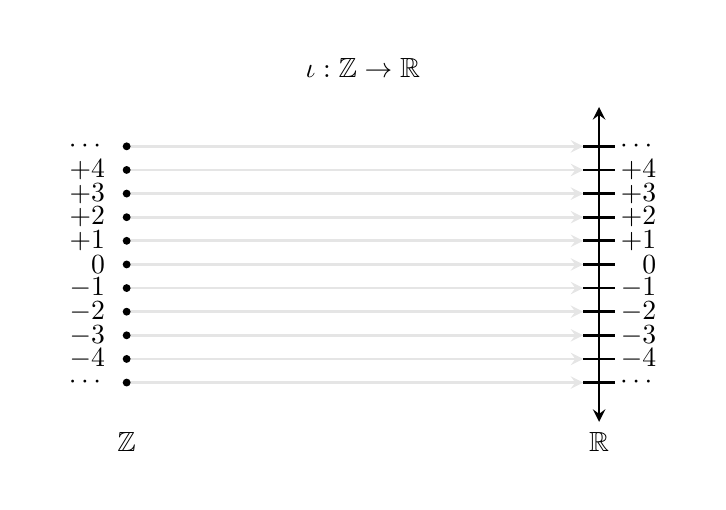
\begin{tikzpicture}[scale=1]

  \draw[white] (-4.25, -2.75) rectangle (4.25, 3);
  
  \node at (0, 2.5) { $\iota: \mathbb{Z} \rightarrow \mathbb{R}$ };

  \foreach [count=\n] \y in {-1.5, -1.2, ..., 1.51} {
    \draw[gray90, ->, >=stealth, line width=1] (-3, \y) -- (2.8, \y);
  }
  
  \node at (-3, -2.25) { $\mathbb{Z}$ };
  
  \draw[<->, >=stealth, line width=1] (3, -2) -- (3, 2);
  \node at (3, -2.25) { $\mathbb{R}$ };
 
  \foreach [count=\n] \y in {-1.5, -1.2, ..., 1.8} {
    \fill (-3, \y) circle (0.05);
    \draw[line width=1] (2.8, \y) -- (3.2, \y);
  }
  
  \foreach [count=\n] \y in {0.3, 0.6, ..., 1.3} {
    \pgfmathtruncatemacro{\m}{\n};
    \node at (-3.5, \y) { $+\m$ };
    \node at (+3.5, \y) { $+\m$ };
  }
  
  \foreach [count=\n] \y in {-1.2, -0.9, ..., 0.0} {
    \pgfmathtruncatemacro{\m}{\n - 5};
    \node at (-3.5, \y) { $\m$ };
    \node at (+3.5, \y) { $\m$ };
  }
  
  \node at (-3.5, +1.5) { $\cdots$ };
  \node at (-3.5, -1.5) { $\cdots$ };
  \node at (-3.5, 0) { $\hphantom{+}0$ };
  \node at (+3.5, 0) { $\hphantom{+}0$ };
  \node at (+3.5, +1.5) { $\cdots$ };
  \node at (+3.5, -1.5) { $\cdots$ };
 
\end{tikzpicture}

\end{document}  